\section{Ferramentas}

Para desenvolver código para o aplicativo, foi usado o Android Studio (Figura \ref{devfig02}), a IDE mais popular para esta tarefa, recomendada pelo próprio Google. Já para a API REST foi usado o editor de texto Atom (Figura \ref{devfig02}).

\begin{figure}[ht!]
	\centering
    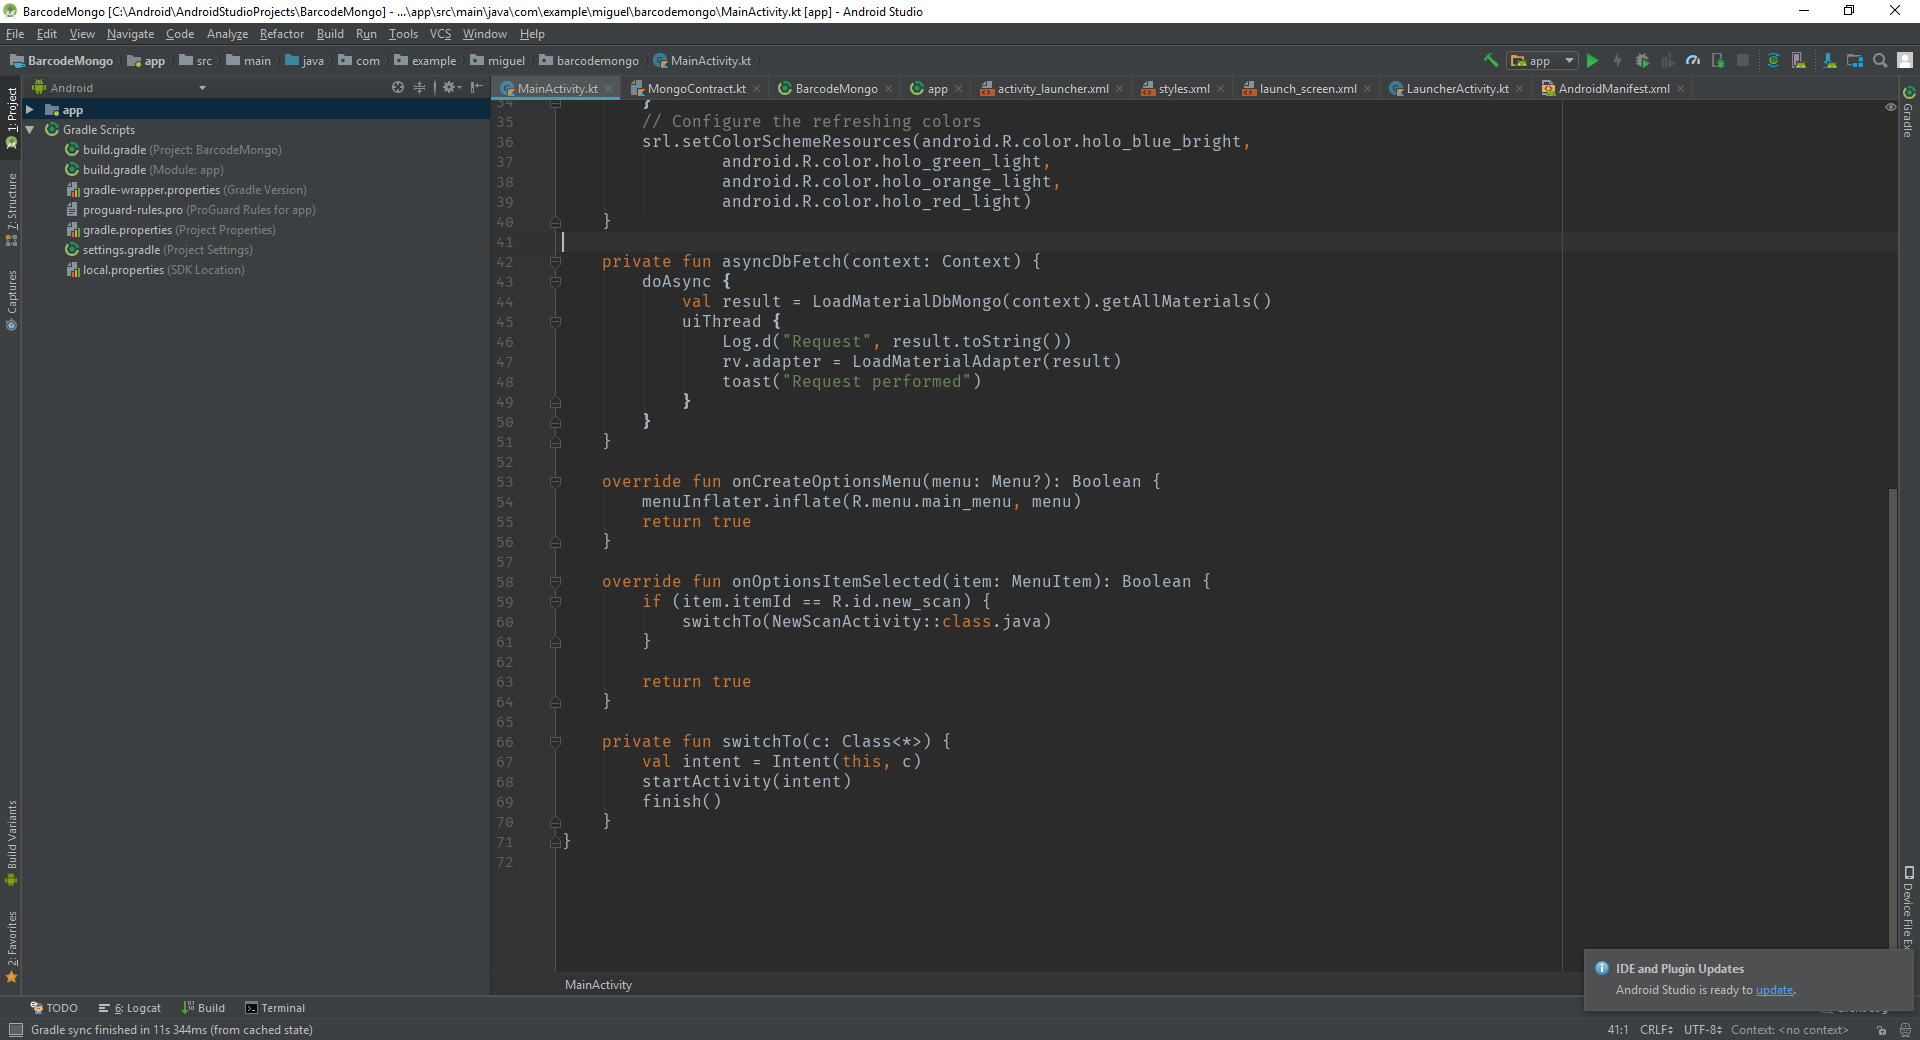
\includegraphics[width=\textwidth]{Cap3/androidstudio}
    \caption{Interface do Android Studio}
    \label{devfig01}
\end{figure}

\begin{figure}[ht!]
	\centering
    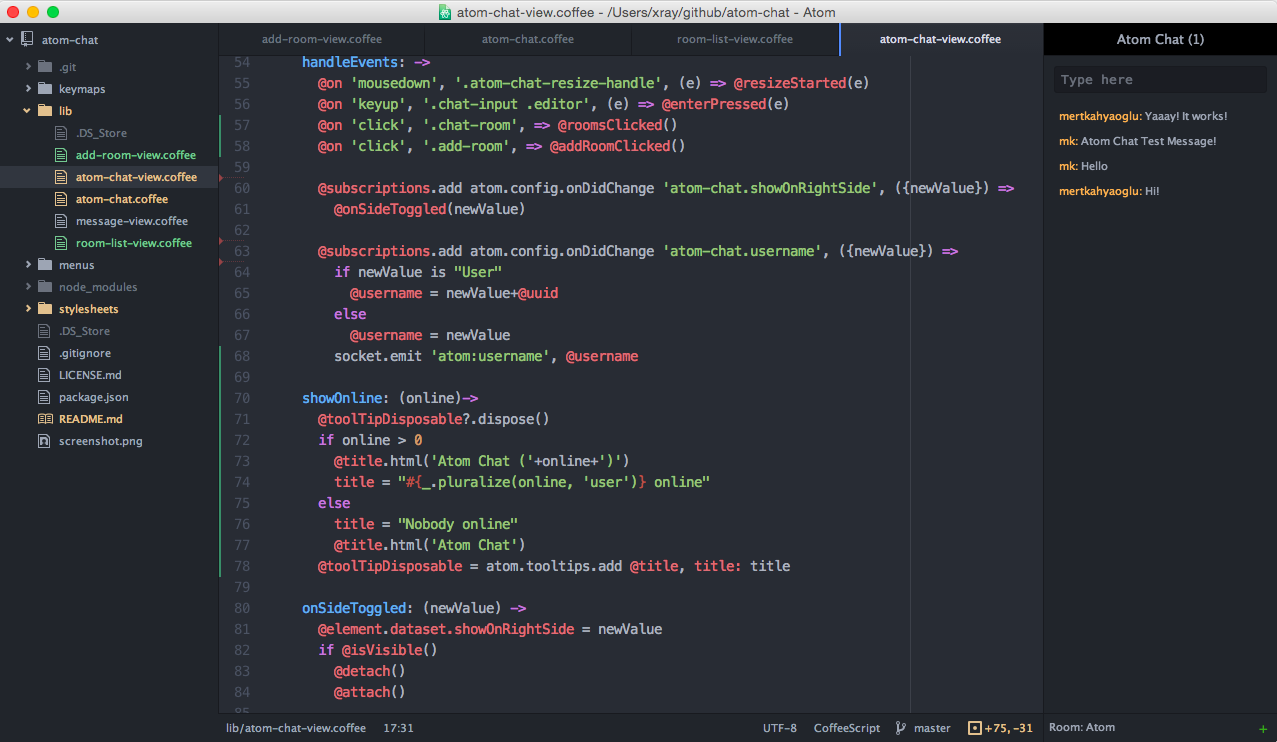
\includegraphics[width=\textwidth]{Cap3/atom}
    \caption{Interface do Atom}
    \label{devfig02}
\end{figure}

\section{Protótipo 1 - BarcodeTest}

Este protótipo não chega a usar a API REST, que ainda não tinha sido feita. Ele é fortemente baseado no projeto que foi ensinado no curso \cite{kotlinandroid}, chamado HabitTrainer, mostrado na Figura \ref{devfig03}.

A Figura \ref{devfig03:figa} mostra um padrão de design Android chamado \textit{Recycler view}. Ele cria uma estrutura de cartões que otimiza o uso de memória por reciclar elementos que já estão na tela para produzir outros semelhantes. Tal estrutura foi usada no BarcodeTest para exibir os elementos cujo código de barras foi lido.

A figura \ref{devfig03:figb} mostra a tela de criação de novos hábitos no HabitTrainer. Este aplicativo usa a própria memória do celular com o padrão SQLite, que é portátil e fica armazenado no próprio celular. O BarcodeTest usa o mesmo modelo de banco de dados.

\begin{figure}[ht!]
	\centering
    \subfloat[Tela inicial][Tela inicial]{
    	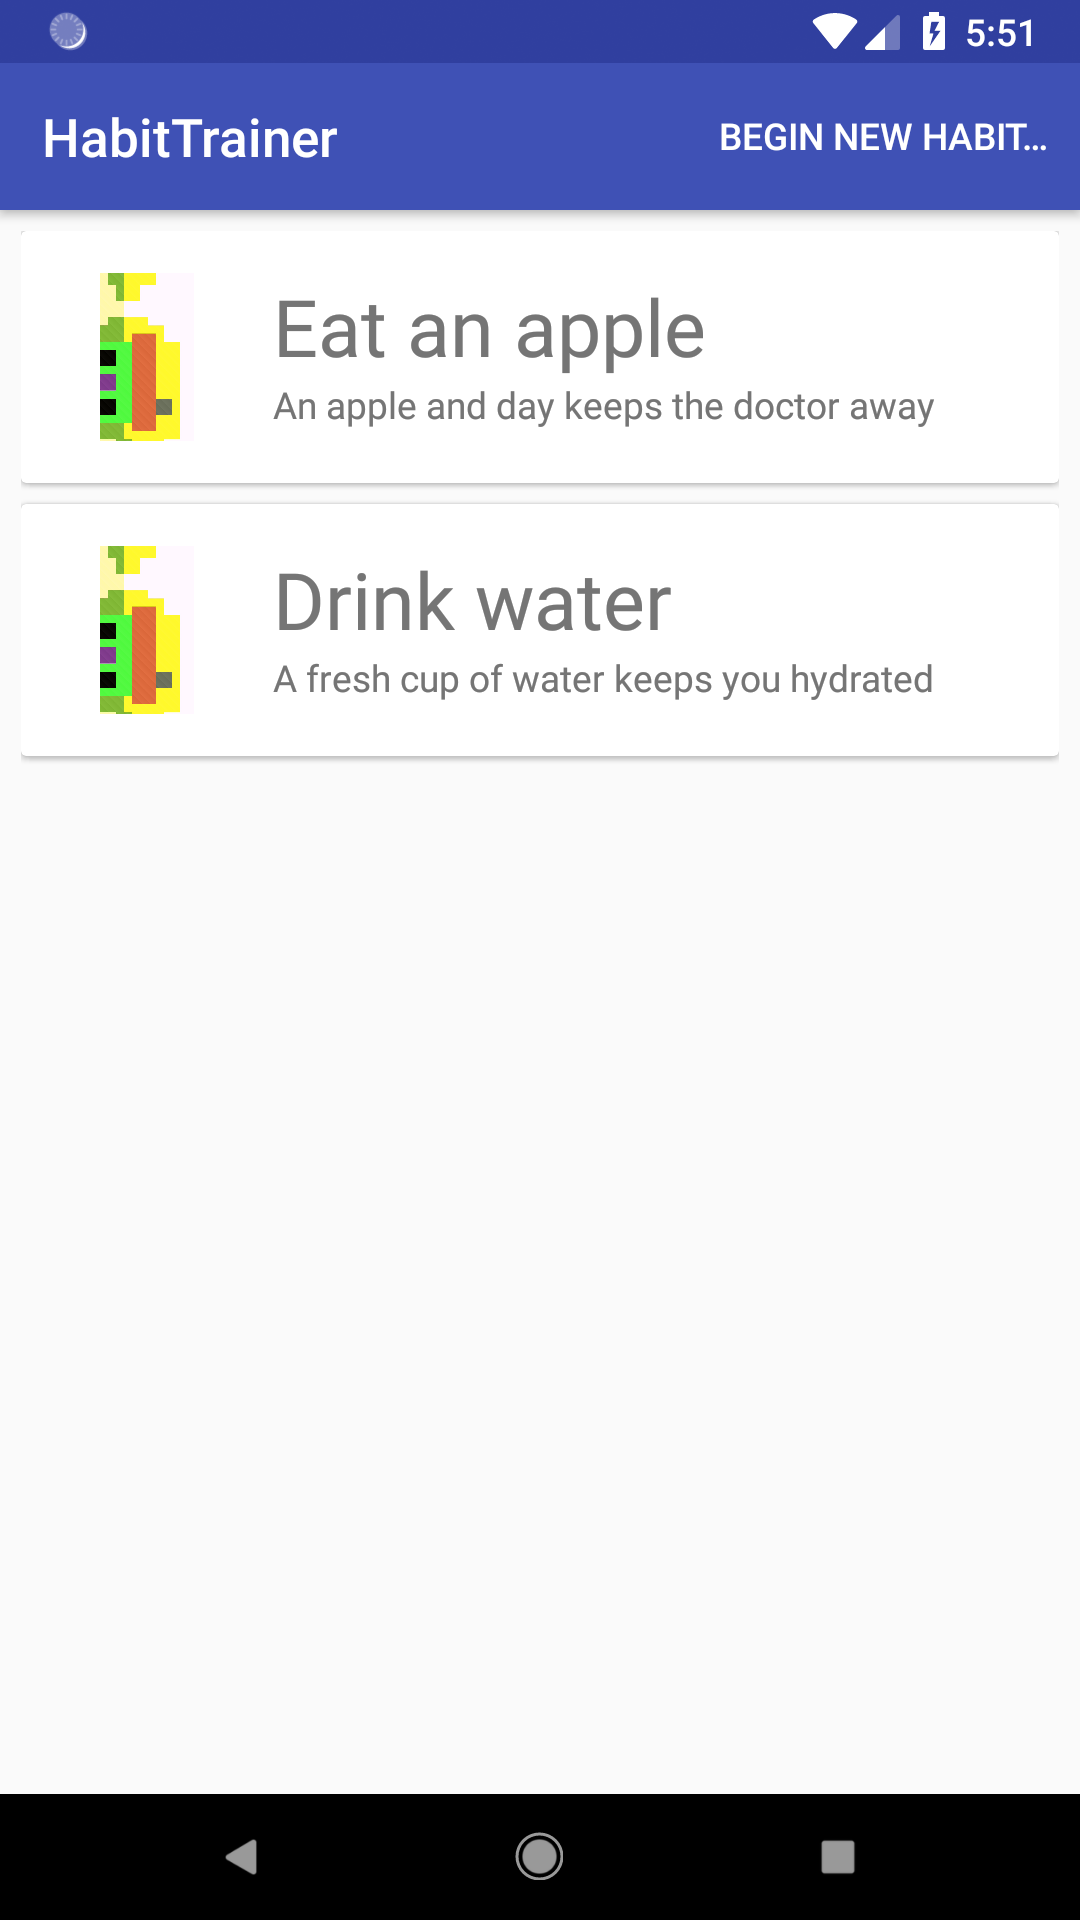
\includegraphics[width=0.4\textwidth]{Cap3/habittrainer}
        \label{devfig03:figa}
    }
    \quad
    \subfloat[Adicionar novo hábito][Adicionar novo hábito]{
    	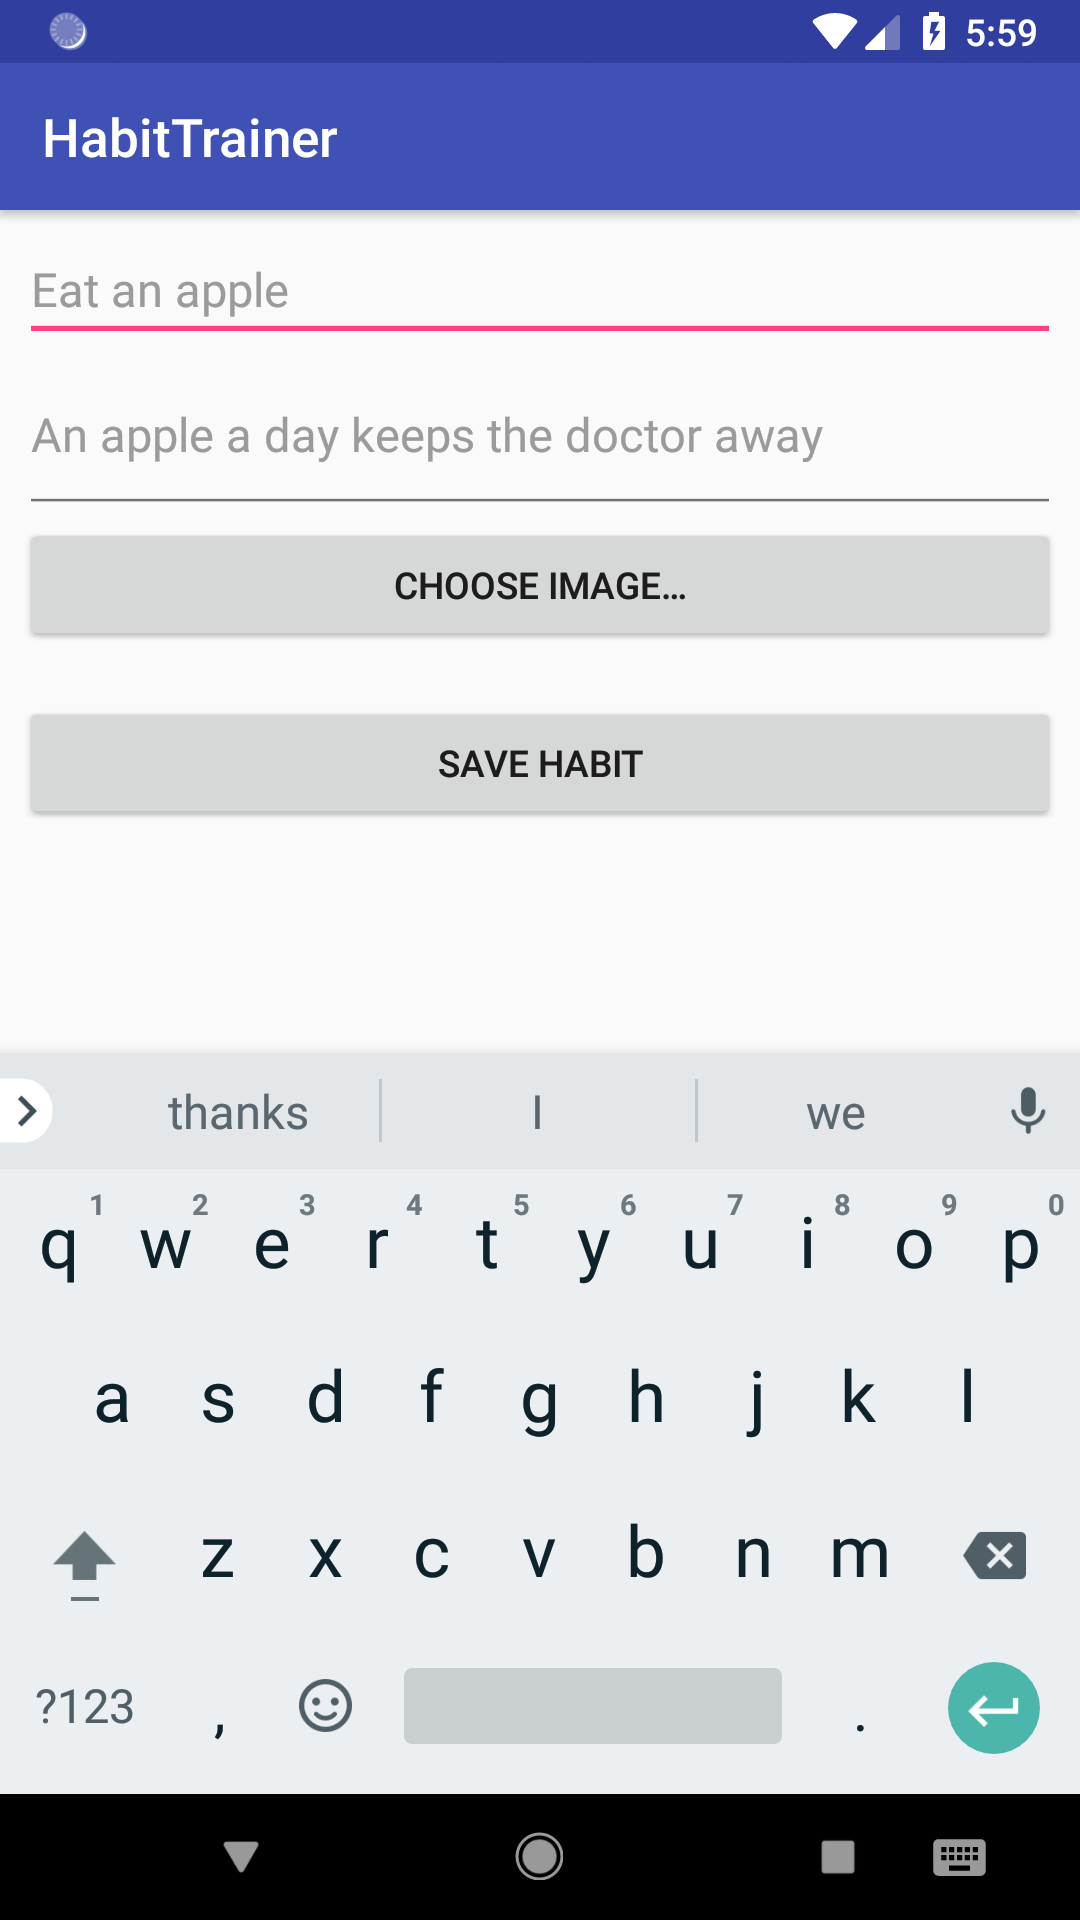
\includegraphics[width=0.4\textwidth]{Cap3/habittrainerbegin}
        \label{devfig03:figb}
    }
    \caption{Aplicativo HabitTrainer}
    \label{devfig03}
\end{figure}

\subsection{Código}

O BarcodeTest consiste de 3 \textit{Activities}, isto é, 3 ``telas'' diferentes, mostradas na Figura \ref{devfig04}. Cada uma delas será discutida a seguir.

\begin{figure}[ht!]
	\centering
    \subfloat[Tela inicial][Tela inicial]{
    	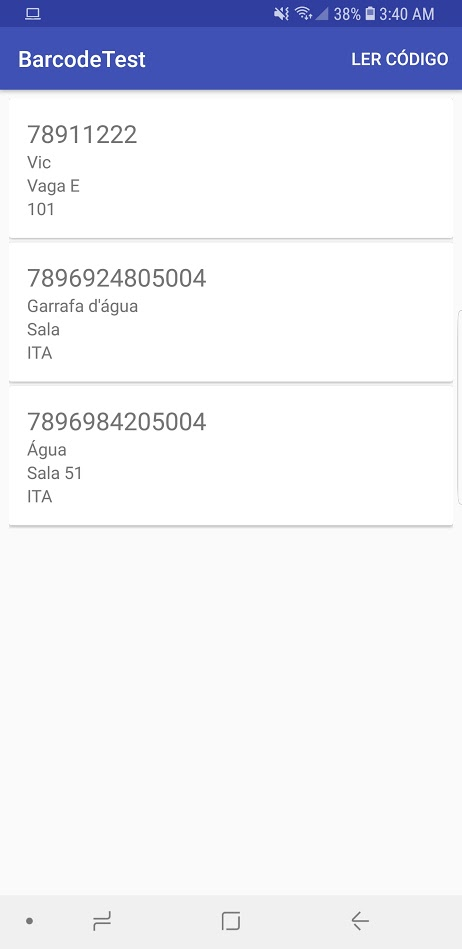
\includegraphics[width=0.3\textwidth]{Cap3/barcodetest}
        \label{devfig04:figa}
    }
    \quad
    \subfloat[Leitor de código de barras][Leitor de código de barras]{
    	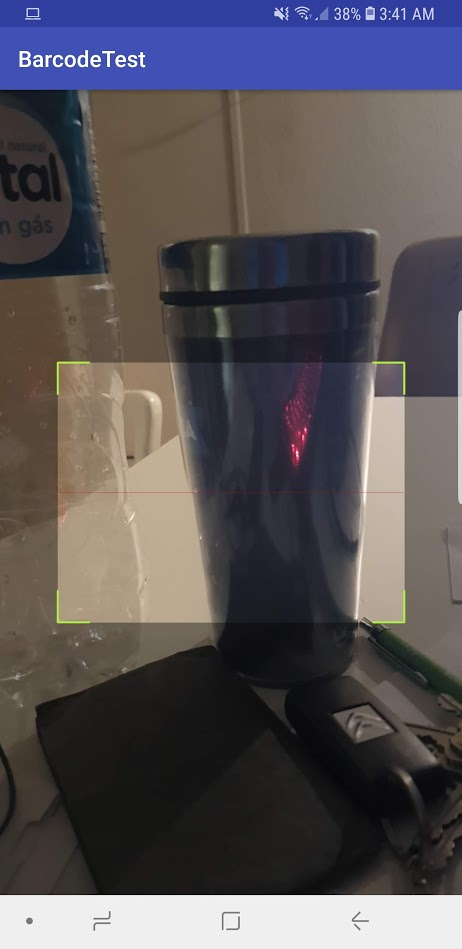
\includegraphics[width=0.3\textwidth]{Cap3/barcodetestread}
        \label{devfig04:figb}
    }
    \qquad
    \subfloat[Inserindo os dados do material][Inserindo os dados do material]{
    	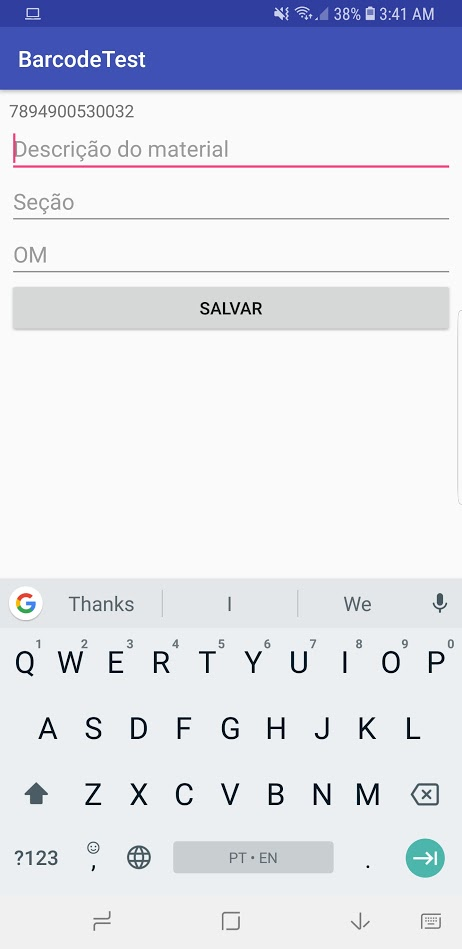
\includegraphics[width=0.3\textwidth]{Cap3/barcodetestinput}
        \label{devfig04:figc}
    }
    \quad
    \subfloat[Mensagem de erro][Mensagem de erro]{
    	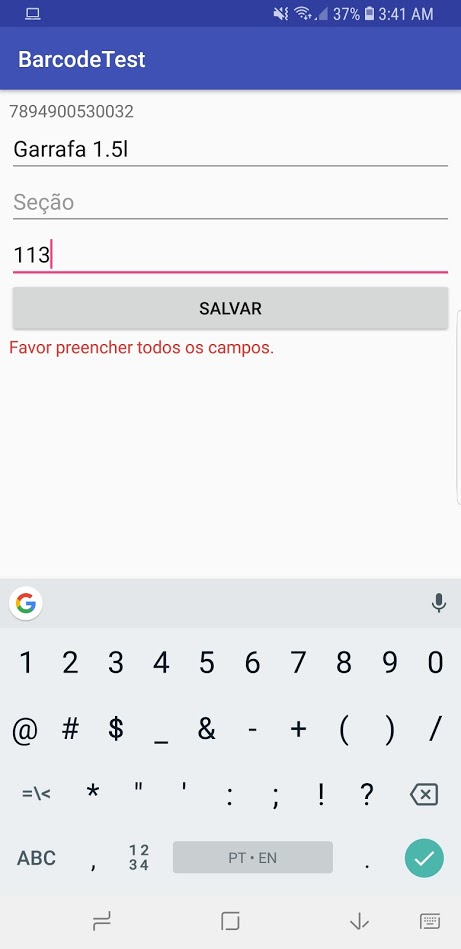
\includegraphics[width=0.3\textwidth]{Cap3/barcodetesterror}
        \label{devfig04:figd}
    }
    \caption{Aplicativo BarcodeTest}
    \label{devfig04}
\end{figure}

\subsubsection*{\textit{MainActivity.kt}}

A \textit{MainActivity} (Figura \ref{devfig04:figa}) contém o padrão \textit{Recycler view} já citado, mostrando cartões para cada um dos códigos que foram lidos e salvos. Cada cartão representa um objeto da classe \textit{LoadMaterial.kt}, cujo código é descrito a seguir. Nesse código, pode-se ver uma das grandes vantagens de Kotlin com relação a Java, as \textit{data classes}. Elas provêm código pronto para \textit{getters}, \textit{setters}, \textit{toString} e outras funções que em Java seria necessário digitar uma a uma.

\begin{minted}[
frame=lines,
framesep=2mm,
baselinestretch=1.2,
fontsize=\footnotesize,
linenos,
label=LoadActivity.kt
]{kotlin}
package com.example.miguel.barcodetest

data class LoadMaterial(val code: String,
                        val description: String,
                        val section: String,
                        val mo: String)
\end{minted}

Nesse ponto, ainda não se usa a especificação de que as OMs e seções possuem um código numérico. Fica como o usuário digitou. A base de dados é especificada de acordo com o seguinte código SQL:

\begin{minted}[
fontsize=\footnotesize
]{sql}
CREATE TABLE material (id TEXT PRIMARY KEY, description TEXT, section TEXT, mo TEXT)
\end{minted}

Dessa forma, o id é o código de barras e, por ele ser único, ele é definido como chave primária da tabela. Para facilitar a leitura, armazenamento e comparação dos códigos, optou-se por colocar o código de barras como texto em vez de número.

Quando o usuário aperta o botão ``LER CÓDIGO'' no canto superior direito, a atividade é finalizada e inicia-se a atividade \textit{NewScanActivity}. Essa finalização é importante para atualizar a lista de cartões no caso de um novo código de barras ser lido e armazenado. Além disso, por causa da finalização que foi colocada tanto nessa quanto nas outras atividades, o botão de voltar quando apertado nessa tela sempre fecha o aplicativo.

\subsubsection*{\textit{NewScanActivity.kt}}

A \textit{NewScanActivity} (Figura \ref{devfig04:figb}) utiliza a biblioteca \textit{open-source} ZBarScanView, que possibilita a leitura dos códigos usando a caixa e a linha. É importante notar que para usar a câmera de um celular Android com um aplicativo, precisa-se pedir acesso explicitamente no arquivo \textit{AndroidManifest.xml} do projeto, da seguinte maneira:

\begin{center}
\mint{xml}|<uses-permission android:name="android.permission.CAMERA" />|
\end{center}

Ao ler um código de barras, esta atividade fecha e envia o número lido para a \textit{StoreScanActivity}. Se o botão de voltar for pressionado, esta atividade finaliza e o aplicativo abre uma nova \textit{MainActivity}.

\subsubsection*{StoreScanActivity}

A \textit{StoreScanActivity.kt} (Figura \ref{devfig04:figc}) recebe o código lido na \textit{NewScanActivity}. Tal código pode ser visto acima das caixas de texto. Ele é escrito para que o usuário confirme que o código foi lido corretamente, já que o leitor pode ter sido mal-posicionado em relação ao código ou algo do tipo. Com os dados inseridos, o botão ``SALVAR'' armazena o código na base de dados de acordo com o modelo que foi descrito.

Há duas funcionalidades importantes nesta atividade. A primeira é que, ao ler um código que já está salvo na base de dados, os campos que o usuário deve preencher já vêm preenchidos com o conteúdo armazenado relacionado a esse código, dando ao usuário a opção de atualizar os valores em vez de sobre-escrevê-los. Isto resolve o erro que poderia ser causado ao tentar salvar duas linhas na tabela com a mesma chave primária. A segunda é demonstrada na Figura \ref{devfig04:figd}, e consiste de exibir uma mensagem de erro caso algum dos campos esteja vazio, tornando assim os campos obrigatórios.

Ao salvar, esta atividade é finalizada e o aplicativo abre uma nova \textit{MainActivity}. Por outro lado, se o botão de voltar for pressionado, esta atividade finaliza e uma nova \textit{NewScanActivity} é aberta.

\subsection{Protótipo 2 - BarcodeMongo}

A grande diferença deste para o BarcodeTest é a inclusão da API REST. Aqui, é usada uma máquina virtual com Ubuntu 16.04 como servidor remoto. Usando a rede local, 

% This chapter explains how to set up SITL ArduPilot Simulator in a virtual machine environment on Windows following the instructions the Ardupilot Dev Team tutorial. The tutorial was tested on Windows 10 with Oracle VM VirtualBox 5.2.12 and Ubuntu 16.04.
% %http://ardupilot.org/dev/docs/setting-up-sitl-on-linux.html

% Software In The Loop simulator allows to run ArduPilot code without any hardware. So SITL simulation is ideal to test new featues and changes in the code during development.

% \section{Downloading the ArduPilot Code} \label{downloading_the_code}
% %http://ardupilot.org/dev/docs/setting-up-sitl-on-linux.html
% The ArduPilot project uses git for source code management and GitHub for source code hosting. To install git use the commands in the terminal:  %http://ardupilot.org/dev/docs/where-to-get-the-code.html#where-to-get-the-code

% \begin{verbatim}
% sudo apt-get update
% sudo apt-get install git
% \end{verbatim}

% Now you have to get a copy of the ardupilot git repository. Open the terminal and run:
% \begin{verbatim}
% git clone git://github.com/ArduPilot/ardupilot.git
% cd ardupilot
% git submodule update --init --recursive
% \end{verbatim}

% Install required packages using the script \textit{install-prereqs-ubuntu.sh}  located in \textit{ardupilot/Tools/scripts}. Go to the directory you cloned ardupilot into and use the following command line. It can take a while depending on your internet connexion. Don't forget to accept the changes when asked.
% \begin{verbatim}
% cd ardupilot/Tools/scripts/install-prereqs-ubuntu.sh
% \end{verbatim}

% Now you have to add the following lines to the end of your \textit{.bashrc} file in your home directory. Notice the . on the start of that filename. Also, this is a hidden file, so if you’re using a file manager, make sure to turn on “show hidden files”.

% \begin{verbatim} 
% export PATH=$PATH:$HOME/ardupilot/Tools/autotest
% export PATH=/usr/lib/ccache:$PATH
% \end{verbatim}

% Save the \textit{.bashrc} file and open the terminal. Then reload your PATH by using the “dot” command in a terminal:

% \begin{verbatim} 
% . ~/.bashrc
% \end{verbatim}
% If you don't change the  \textit{.bashrc} file you will not be able to use \textit{sim\_vehicle.py} as described in the next section.

% \section{How to start SITL simulator}
% In the terminal, go to the directory of the vehicle you want to make a simulation with. For example, for the multicopter code use the command line:
% \begin{verbatim}
% cd ardupilot/ArduCopter
% \end{verbatim}

% Then start the simulator using \textit{sim\_vehicle.py}. The first time you run it you should use the -w option to wipe the virtual EEPROM and load the right default parameters for your vehicle.
% \begin{verbatim}
% sim_vehicle.py -w
% \end{verbatim}

% After the default parameters are loaded you can start the simulator normally. First kill the sim\_vehicle.py you are running using Ctrl-C. Then:
% \begin{verbatim}
% sim_vehicle.py --console --map
% \end{verbatim}

% \section{FlightGear 3D View}  \label{sec_flightgear_view}

% It is possible to install FlightGear Flight Simulator to display a 3D simulation of the vehicle and its surroundings. To install FlightGear from terminal use next command line. It may take a few minutes to finish the download.

% \begin{verbatim}
% sudo apt-get install flightgear
% \end{verbatim}

% If you want to run the simulation including the FlightGear 3D view, you need to open a new terminal, go to the directory \textit{/ardupilot/Tools/autotest/} and open \textit{fg\_quad\_view.sh} (Copter). This will start FlightGear. The next steps show the procedure to run the simulation.

% \begin{enumerate}
% \item In a terminal use the command lines:
% \begin{verbatim} 
% cd ardupilot/Tools/autotest
% ./fg_quad_view.sh 
% \end{verbatim}

% \item In other terminal:
% \begin{verbatim} 
% cd ardupilot/Ardu
% sim_vehicle.py -j4 -L KSFO --map --console
% \end{verbatim}

% \end{enumerate}

% In the step 2, KSFO indicates the location where the simulation will take place. FlightGear will always start by loading scenery at KSFO (San Francisco International Airport) but will change to the selected scenery once SITL is started.
% If the vehicle appear to be hovering in space (no scenery) then you don't have the files for that location, but you can download it after. 

% \subsection{Adding a new location to FlightGear}
	
%     New locations are hard-coded into a file. This section shows how to add a new location. We will call the location as KSFO\_PAPI, because it will be next to PAPI lights in a lane of KSFO.
    
%     In the directory \textit{ardupilot/Tools/autotest} find the \textit{locations.txt} file. This file contains all the locations you can choose for simulation. Each line follows the sintaxe:

% \begin{verbatim}
% #NAME=latitude,longitude,absolute-altitude,heading
% \end{verbatim}  

% Then add to the file the next line. 
% \begin{verbatim}
% KSFO_PAPI = 37.6136, -122.357, 5.3, 297.9
% \end{verbatim}  
% When you run the simulation in KSFO\_PAPI location using the steps shown in section \ref{sec_flightgear_view}, FlightGear environment will be as in figure \ref{fig_papi_lights}.

% \begin{figure}[ht!] 
% \centering
% 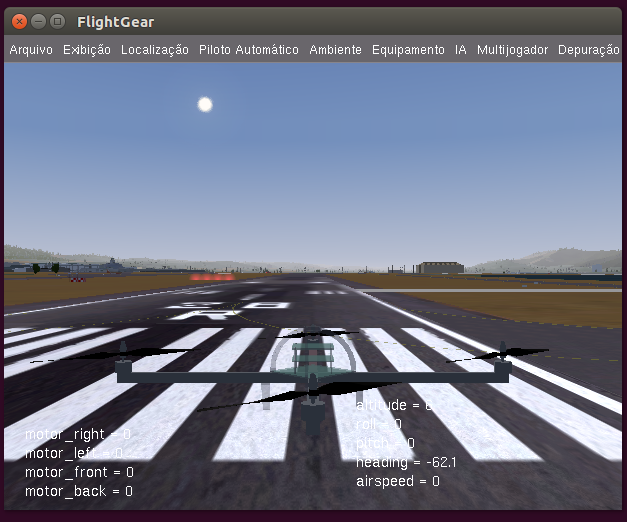
\includegraphics[width=1.0\textwidth]{Cap3/fig_papi_lights}
% \caption{Image from FlightGear simulator running in SITL. Observe four red lights (PAPI) in the left of the lane. }
% \label{fig_papi_lights}
% \end{figure}




